\documentclass{beamer}
\usetheme{Madrid}

\usepackage{amsmath, amssymb, amsthm}
\usepackage{graphicx}
\usepackage{listings}
\usepackage{gensymb}
\usepackage[utf8]{inputenc}
\usepackage{hyperref}
\usepackage{gvv}
\usepackage{tikz}
\usepackage{minted}
\usetikzlibrary{decorations.pathmorphing}

\begin{document}

\title{1-1.6.29}
\author{AI24BTECH11013 - Geetha charani$^{*}$}
\date{}
\frame{\titlepage}

\begin{frame}
\frametitle{Question}
Show that the points A\brak{2, 3, -4}, B\brak{1, -2, 3} and C\brak{3, 8, -11} are collinear.
\end{frame}
\begin{frame}{allowframebreaks}
\frametitle{Solution}
Given,\\
    A = \myvec{2 \\ 3\\ -4}, B = \myvec{1 \\ -2 \\ 3}, C = \myvec{3 \\ 8 \\ -11}\\ 
    For Points $\Vec{A}, \Vec{B}, \Vec{C}$ to be collinear if\\
    \begin{align}
        rank \myvec{\Vec{B}-\Vec{A} & \Vec{C}-\Vec{A}}\\
        \Vec{B}-\Vec{A} = \myvec{1 \\ -2 \\ 3} - \myvec{2 \\ 3\\ -4}\\
        = \myvec{-1 \\ -5 \\ 7}
    \end{align}
\end{frame}
\begin{frame}
\frametitle{Solution}
\begin{align}
        \Vec{C} - \Vec{A} = \myvec{3 \\ 8 \\ -11} - \myvec{2 \\ 3\\ -4}\\
        =\myvec{1 \\ 5 \\ -7}\\
        Rank \myvec{\Vec{B}-\Vec{A} & \Vec{C}-\Vec{A}} = \myvec{-1 & 1 \\ -5 & 5 \\ 7 & -7}\\
         rank\myvec{-1 & 1 \\ -5 & 5 \\ 7 & -7} = 1
    \end{align}
    \end{frame}
    \begin{frame}
    Since, the rank of \myvec{\Vec{B}-\Vec{A} & \Vec{C}-\Vec{A}} = 1. Therefore, A = \myvec{2 \\ 3\\ -4}, B = \myvec{1 \\ -2 \\ 3}, C = \myvec{3 \\ 8 \\ -11} are collinear.
\end{frame}
\begin{frame}[fragile]
\frametitle{Figure}
\begin{figure}
    \centering
    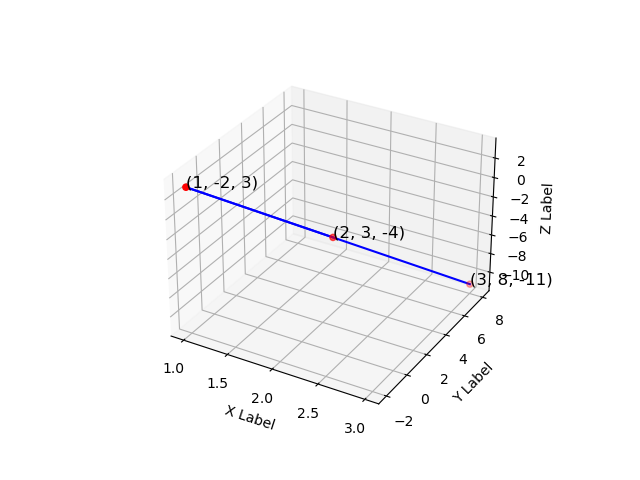
\includegraphics[width=0.90\linewidth]{figs/fig_1.png}
    \label{fig:enter-label}
\end{figure}
\end{frame}
% Define colors for syntax highlighting               \definecolor{codegreen}{rgb}{0,0.6,0}                 \definecolor{codegray}{rgb}{0.5,0.5,0.5}              \definecolor{codepurple}{rgb}{0.58,0,0.82}            \definecolor{backcolour}{rgb}{0.95,0.95,0.92}                                                              % Python style for highlighting                      \lstset{                                            102     language=Python,                                103     basicstyle=\ttfamily\small,                     104     keywordstyle=\color{blue},
%  stringstyle=\color{codepurple},
 %  commentstyle=\color{codegreen}
 %  backgroundcolor=\color{backcolour},
  % breaklines=true,
   %breakatwhitespace=true,
   %tabsize=4

 \begin{frame}[fragile,allowframebreaks]
 \frametitle{Python Code}
 \lstinputlisting[label=mycode]{codes/collinear.py}
\end{frame}
\begin{frame}
\frametitle{C code}
    \lstinputlisting[label=mycode]{codes/main.c}
    \label{fig:enter-label}
\end{frame}
\end{document}

